\section{Durchführung}
\label{sec:durchführung}

Eine schematische Darstellung des Versuchsaufbaus findet sich in \autoref{fig:aufbau}.

\begin{figure}[H]
    \centering
    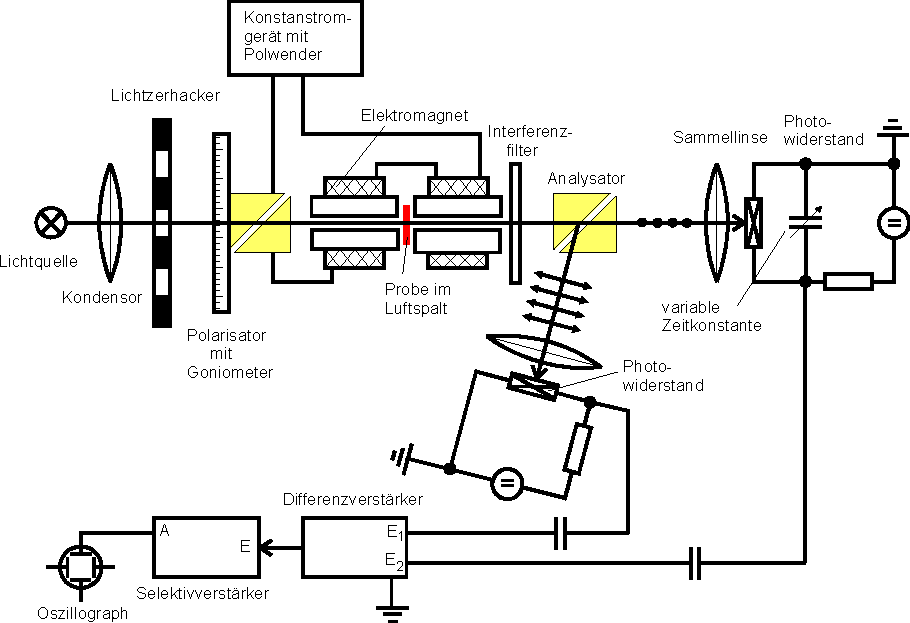
\includegraphics{figures/Aufbau.pdf}
    \caption{Schematischer Aufbau des Versuches \cite{v46}.}
    \label{fig:aufbau}
\end{figure}

Von einer Halogenlampe wird dabei Licht emittiert. Dieses wird durch eine Kondensorlinse fokussiert und durch ein Glan-Thompson-Prisma linear polarisiert.
Die Kondensorlinse hat darüber hinaus die Aufgabe, einen parallelen Strahlengang zu gewährleisten, da die Lampe prinzipiell Licht in alle Richtungen aussendet.
Das nun linear polarisierte Licht fällt nun durch die Probe im Elektromagneten.
Damit dort ein Magnetfeld herrschen kann, befindet sich die Probe in einem Luftspalt im Magneten.
Nach dem Verlassen des Elektromagneten passiert das Licht einen Interferenzfilter, der nur die gewünschte infrarote Wellenlänge herausfiltert und
trifft auf ein weiteres Glan-Thompson-Prisma.
Dort wird es in zwei Lichtstrahlen aufgespalten und durch Sammellinsen auf zwei unterschiedliche Photowiderstände abgebildet.
Die an den beiden Widerständen abfallenden Spannungen werden an einen Differenzverstärker gekoppelt.
Um eine möglichst gute Rauschunterdrückung sicherzustellen, wird das Licht vor dem Durchgang durch den Magneten von einem Lichtzerhacker in kürzere Pulse zerteilt,
sodass mittels eines Selektivverstärkers die Frequenz des Choppers verstärkt werden kann.

\subsection{Justierung der Apparatur}

Vor der eigentlichen Durchführung muss der Strahlengang justiert werden.
Dazu wird zunächst die Abdeckung beider Photowiderstände entfernt.
Es wird sichergestellt, dass bei geeigneter Polarisation die einfallenden Lichtpunkte an beiden Widerständen zum Verschwinden gebracht werden können.
Ist dies nicht der Fall, muss die Rotation der Widerstände angepasst werden, sodass am seitlichen Widerstand der verschwindende der beiden Lichtpulse gewählt wird. \\

Jetzt wird der Zerhacker eingeschaltet und auf eine Frequenz von $\SI{450}{\hertz}$ eingestellt.
Durch Maximierung des Differenzsignals am Oszilloskop wird der Selektivverstärker auf die gewählte Frequenz eingestellt.

Zur abschließenden Justage werden Probe und Interferenzfilter in die Apparatur gesetzt und überprüft, dass bei geeigneter Polarisation das Signal am Oszilloskop
näherungsweise null wird.


\subsection{Messung}

Nun wird das Magnetfeld bei einem Strom von $I = \SI{10}{A}$ eingeschaltet und die Messung begonnen.
Zunächst wird eine n-dotierte GaAs-Probe genutzt.
Der Polarisationswinkel wird für neun verschiedene Interferenzfilter so eingestellt, dass das Signal am Oszilloskop möglichst klein wird.
Anschließend wird das Magnetfeld umgepolt, sodass eine effektive Drehwinkeldifferenz von $2\theta$ entsteht und die Messung für alle Filter wiederholt.
Dieser Prozess wird für eine weitere n-dotierte sowie eine undotierte Probe als Vergleichsmessung erneut durchgeführt. \\

Für den Drehwinkel gilt dann $\theta = \frac{1}{2} (\theta_1 - \theta_2)$.